%!TEX root = ../thesis.tex
\section{Design Guidelines}

Researchers provide different findings on the effectiveness of media formats of software tutorials. Evaluating the instructional potential of videos began in the 1990s. Palmiter, Elkerton \cite{Palmiter:1991:ADV:107792.107797,Palmiter:1993:ADL:1461829.1461830}, and Harrison \cite{Harrison:1995uh} studied the effect of animated demonstrations on learning and instruction recall. More recently, Grabler \ea compared how users followed book tutorials, videos, and automatically generated static tutorials \cite{Grabler:2009jj}. Their results showed that automatically generated text and image tutorials outperformed video or book instructions on time and errors. Grossman \ea studied the effectiveness of embedding short (10-25 second) video clips in applications \cite{Grossman:2010wr}. They found that participants who had access to video-based tooltips were significantly faster in completing tasks than those who viewed static ones.

While these studies suggest that there is still some debate over the trade-offs between step-by-step static and video tutorials, they provide strong support for two key claims: step-by-step tutorials help users make fewer errors by allowing them to work at their own pace, while videos can help provide subtle details of complex interactions that are difficult to represent statically. Based on these findings, we designed a formative user study that investigates whether video clips can be incorporated into a step-by-step framework to help users follow certain types of image-editing tasks within a tutorial.

\subsection{Formative User Study}

\begin{figure*}[t]
  \centering
  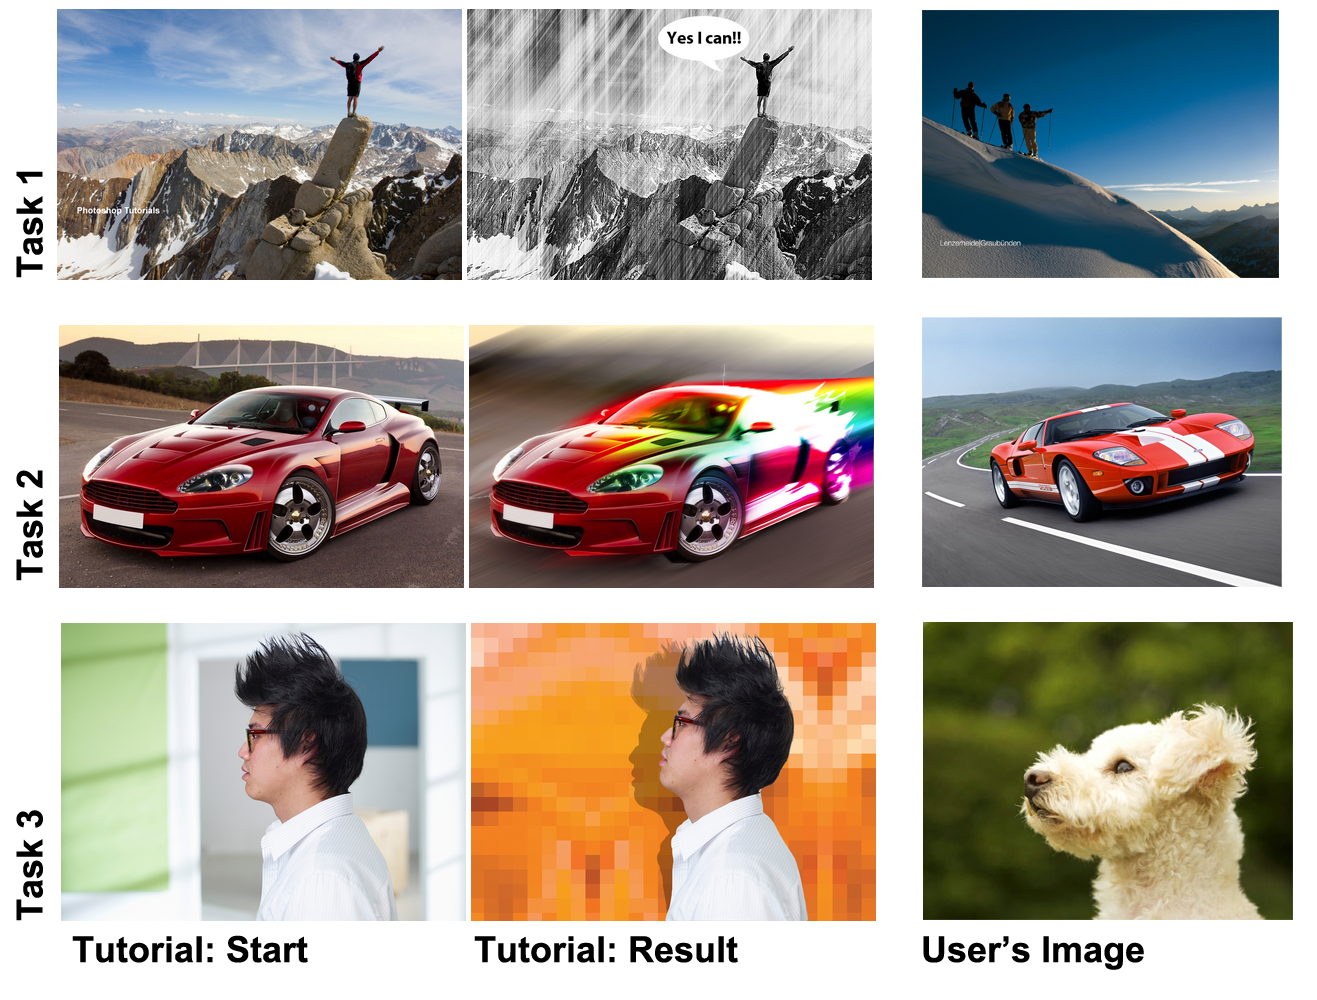
\includegraphics[width=0.8\textwidth]{\mixt/fig/formative_study/study-images}
  \caption{In our formative study, participants completed three tutorials with images similar but not identical to the originals.}
  \label{fig:formative_tasks}
\end{figure*}

\begin{figure*}[t]
  \centering
  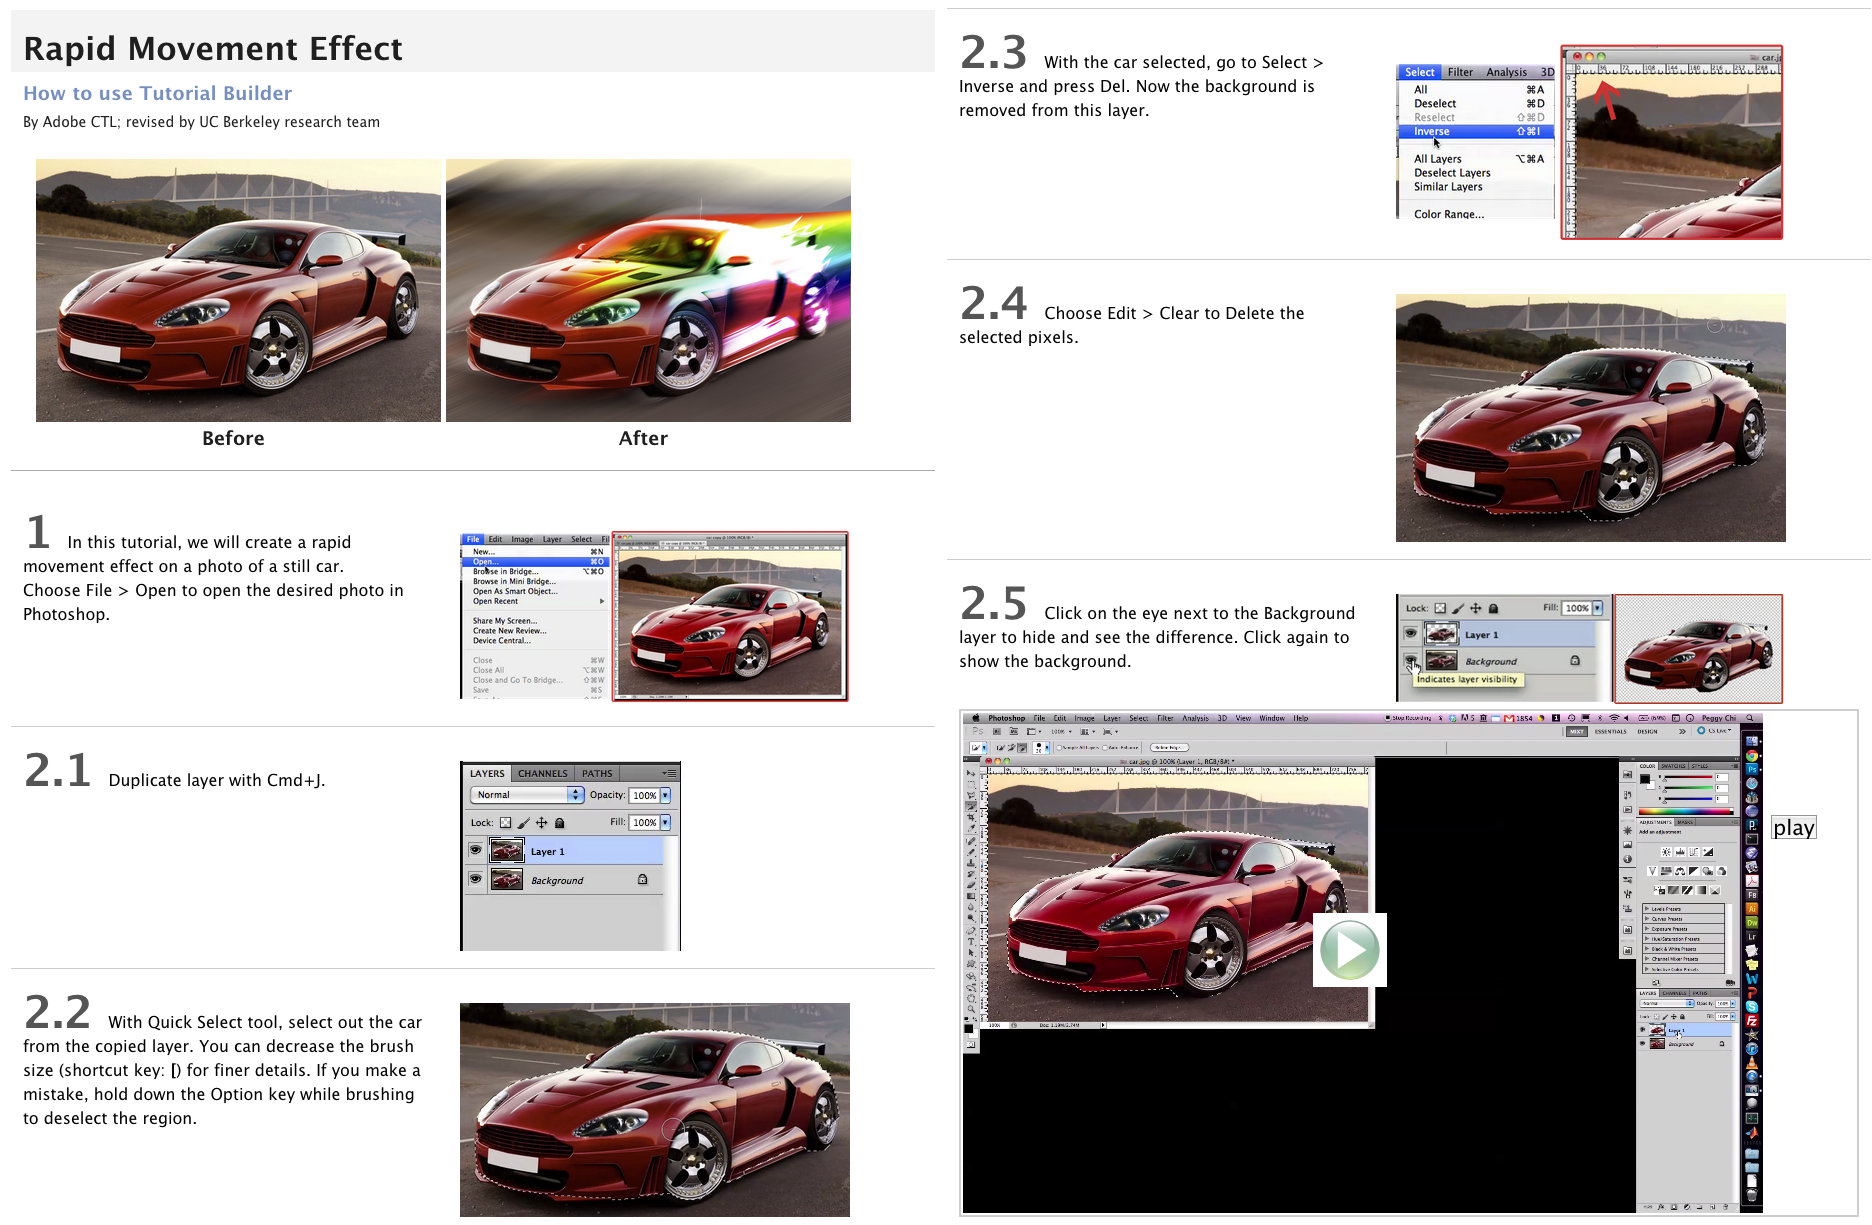
\includegraphics[width=\textwidth]{\mixt/fig/formative_study/study-mixed-example}
  \caption{In the mixed condition, participants saw an HTML page with static images and text; they could expand each step to view a video of that step (here: step 2.5).}
  \label{fig:formative_mixt}
\end{figure*}

% \subsubsection{Study Design}
\subsubsection{Hypothesis}
Our formative study aims to test the following two hypotheses:

H1: Image manipulation tutorials that mix static images and video clips are more effective than all-static or all-video tutorials.

H2: Users benefit more from seeing video clips instead of static text and images for certain types of commands.

\subsubsection{Participants}
We recruited 12 participants (5 males and 7 females, aged 20-52), 4 from a campus student design group and 8 from a computer software company, and compensated each with a \$15 gift card for participating. Our tutorials focused on achieving specific tasks in Adobe Photoshop. We recruited participants who had prior expertise with Adobe Photoshop, but who were not expert users. To demonstrate expertise, potential participants first completed an online screening test that asked them to follow a short image manipulation tutorial and submit the resulting file. The selected participants had between 1 and 20 years of experience using Photoshop.

\subsubsection{Tasks and Material}
The study was based on a within-subject design. We looked through Photoshop books and selected 3 different image manipulation tasks with similar levels of difficulty and complexity (see Figure~\ref{fig:formative_tasks}). Each tutorial comprised 15-20 steps. We focused on tutorials that included new, less common features such as the liquify tool, gradient warp tool, and puppet warp tool to increase the chance that participants would encounter unfamiliar tools. For each tutorial, we created three types of presentations: 1) static (in HTML format displayed on the screen), 2) video (on YouTube with audio narration), and 3) mixed (web interface shown in Figure~\ref{fig:formative_mixt} without audio). To ensure that different formats presented equivalent information where possible, we first recorded and narrated our video tutorials, then manually generated the static version by writing text instructions based on the narration and annotating and cropping frames of the video. To create mixed tutorials we started with the static tutorials and added the corresponding screencapture video segment for each step. To view the video segment for a step in the mixed tutorial, the user had to click on the image for that step. We scaled these videos to a fixed resolution of 800x500 pixels so that at least 2-3 steps would fit on screen when the videos were expanded. Many online tutorials do not offer full-screen resolution videos; even when high-resolution videos are available, they are hard to use as they force users to continually switch between the video and application windows. We disabled the soundtrack in the mixed tutorial to avoid situations when users only relied on auditory instructions instead of learning from static or video formats.

For each task, participants were given a source image that was distinct, but thematically similar to the image manipulated in the tutorial itself. This study design choice was motivated by the fact that users typically want to transfer the techniques found in tutorials to their own images.

\subsubsection{Procedure and Environment}
Each session consisted of 1 warm-up task and 3 experimental tasks. The warm-up task was a short 5-step static tutorial. In the 3 experimental tasks the format and task order were randomized. Each 60-minute session was conducted in a lab environment, using computers running Mac OS X, Adobe Photoshop CS5.1 and a web browser (Google Chrome) for viewing tutorials. Each participant was provided with a keyboard and a mouse and was allowed to adjust the equipment setting such as the monitor position and mouse tracking speed during the warm-up task. Photoshop and the web browser were arranged side-by-side on a 30-inch monitor with a resolution of 2048x1280 pixels. During the study, we used screen capture software to record user performance.

\subsubsection{Measurement}
To evaluate H1, we report the number of errors and repeated attempts that the participants made for each task. While our ultimate goal is skill acquisition and retention, we focus on the pragmatic goal of improving users' success in following tutorials and performing the instructions. We record an error if the participant performed a command incorrectly or skipped a step in the tutorial. While errors give a sense for the effectiveness of the tutorials, they do not measure the extraneous work users might have to perform when they have trouble understanding the correct outcome of a step. For example, if a user makes an error and then correctly executes several steps before recognizing the problem, we count this as a single error, even though the user must go back to fix the problem and then redo the subsequent steps. In addition, users may select the right command, but be dissatisfied with the result of their image and try again (e.g., redrawing a gradient). In such cases, we record all executions of the same step following the first attempt as a repeated attempt. Note that we do not count adjustments of continuous parameters or refinements of selection regions as repeated attempts because in these cases, the user is focusing on a single action rather than repeating a previously executed step. We do count a repeated attempt if the user entirely undoes a step to then retry it.

To evaluate H2, we count the number of different users who click on the video for each step in the mixed tutorials. To determine whether some types of commands benefit from videos more than others, we bin each step into one of the following five command categories based on the types of user interaction and UI elements it involves: brushing/drawing, manipulating control points (e.g., mesh-based warping, spline editing), parameter adjustment (e.g. using a slider to change opacity), UI navigation (e.g., switching tools, finding menu items), and layer operations.

We also collect qualitative data by observing how users follow the presented information and obtain additional feedback via 5-point Likert-scale questions (e.g., ``The {\textless}condition{\textgreater} tutorial was easy to follow.'') and open-ended questions (e.g., ``Compared with static tutorials, what were the pros and cons of the mixed media tutorial?'').
